\documentclass[english]{revcoles}
\usepackage{bookmark}

\setcounter{tocdepth}{5}
\setcounter{secnumdepth}{5}
 %Esto quita el punto final en la numeracion de cada seccion
\usepackage{tocloft}

\usepackage{titlesec}

\titleformat{\subsection}
{\large\bfseries}{\thesubsection}{0.5em}{}
\titleformat{\subsubsection}
{\normalsize\bfseries}{\thesubsubsection}{0.5em}{}
\titleformat{\paragraph}
{\normalsize\bfseries}{\theparagraph}{0.5em}{}
\renewcommand\cftsecaftersnum{}
\renewcommand\thesection{\arabic{section}}
\renewcommand\thesubsection{\thesection.\arabic{subsection}}

\usepackage{scalerel}
\usepackage{tikz}
\usetikzlibrary{svg.path,babel,positioning,shapes.multipart,calc,arrows.meta}

\definecolor{orcidlogocol}{HTML}{A6CE39}
\tikzset{
  orcidlogo/.pic={
    \fill[orcidlogocol] svg{M256,128c0,70.7-57.3,128-128,128C57.3,256,0,198.7,0,128C0,57.3,57.3,0,128,0C198.7,0,256,57.3,256,128z};
    \fill[white] svg{M86.3,186.2H70.9V79.1h15.4v48.4V186.2z}
                 svg{M108.9,79.1h41.6c39.6,0,57,28.3,57,53.6c0,27.5-21.5,53.6-56.8,53.6h-41.8V79.1z M124.3,172.4h24.5c34.9,0,42.9-26.5,42.9-39.7c0-21.5-13.7-39.7-43.7-39.7h-23.7V172.4z}
                 svg{M88.7,56.8c0,5.5-4.5,10.1-10.1,10.1c-5.6,0-10.1-4.6-10.1-10.1c0-5.6,4.5-10.1,10.1-10.1C84.2,46.7,88.7,51.3,88.7,56.8z};
  }
}

\newcommand\orcidicon[1]{\href{https://orcid.org/#1}{\mbox{\scalerel*{

\begin{tikzpicture}[yscale=-1,transform shape]
\pic{orcidlogo};
\end{tikzpicture}
}{|}}}}

%Paquetes adicionales para ecuaciones, símbolos y figuras
\usepackage{amssymb}
\usepackage{booktabs}
\usepackage{longtable}
\usepackage{array}
\usepackage{multirow}
\usepackage{wrapfig}
\usepackage{float}
\usepackage{colortbl}
\usepackage{pdflscape}
\usepackage{tabu}
\usepackage{threeparttable}
\usepackage{threeparttablex}
\usepackage[normalem]{ulem}
\usepackage{makecell}
\usepackage{xcolor}

\begin{document}

\begin{title}
  \title[maintitle = The Effects of Kurtosis on the Estimation of Structural Equation Modelos Over Different Sample Sizes,
    secondtitle = Efectos de la Kurtosis en la estimación de Modelos de Ecuaciones Estructurales bajo distintos tamaños de muestra,
    shorttitle = Effect of Kurtosis on SEM Estimation]
\end{title}

\begin{authors}
  \author[firstname = César,
    surname = Gamboa-Sanabria,
    numberinstitution = 1,
    affiliation = {School of Statistics, University of Costa Rica},
    email = \href{mailto:info@cesargamboasanabria.com}{\nolinkurl{info@cesargamboasanabria.com}}] \orcidicon{0000-0001-6733-4759}
  \author[firstname = Andrés,
    surname = Arguedas-Leiva,
    numberinstitution = 1,
    affiliation = {School of Statistics, University of Costa Rica},
    email = \href{mailto:andres.arguedasleiva@ucr.ac.cr}{\nolinkurl{andres.arguedasleiva@ucr.ac.cr}}] \orcidicon{0000-0001-6299-052X}
\end{authors}

\begin{institutions}
  \institute[subdivision = {School of Statistics},
    division = Faculty of Economical Sciences,
    institution = University of Costa Rica,
    city = San José,
    country = Costa Rica]
\end{institutions}

\begin{mainabstract}
  Insert your abstract here.
  \keywords{SEM, simulation, kurtosis, lavaan}
\end{mainabstract}

\begin{secondaryabstract}
  Inserte su resumen aquí.
  \keywords{SEM, simulación, kurtosis, lavaan}
\end{secondaryabstract}

\section{Introduction}

\subsection{Antecedentes}

Los Modelos de Ecuaciones Estructurales (en adelante SEM, por sus siglas en inglés) representan un compendio de métodos estadísticos que buscan estimar y examinar las relaciones causales existentes entre varias mediciones fácilmente observables con conceptos más abstractos, denominados constructos, que no pueden ser medidos ni analizados de manera directa. Los SEM trabajan de una manera similar a los modelos de regresión más clásicos, pero representan una mejora pues analizan las relaciones causales lineales entre las variables involucradas al mismo tiempo que los errores de medición \cite{Beran2010}. Para medir estas relaciones causales, los SEM cuentan con dos grandes componentes: 1) el modelo estructural, cuya función es cuantificar las relaciones causales presentes entre cada uno de los constructos planteados desde la teoría; y 2) un modelo de medición, cuyo objetivo último es brindar una descripción acerca de cuáles son los indicadores que sirven para medir los constructos en cuestión \cite{Kaplan2012}.

Los SEM están presentes en multitud de campos de investigación como la psicología, la sociología, las políticas públicas y ciencias relacionadas a la familia \cite{Tarka2018}, además, trabajos como el de \citeasnoun{Golob2003} muestran la aplicación de los SEM en fenómenos económicos, o bien en investigación de mercados como sugieren los trabajos de \citeasnoun{Bagozzi1980} y \citeasnoun{Chin2008}. Según \citeasnoun{Beran2010}, la cantidad de referencias a SEM en 1994 fueron de 164, aumentaron a 343 en el 2000 y llegaron a 742 en el 2009, lo cual es una señal de que muchos investigadores alrededor del mundo están mostrando cada vez más interés en este tipo de estudios, pues representan una potente herramienta para la investigación partiendo de la teoría sustantiva que poseen los diversos estudios.

Uno de los principales campos de aplicación de los SEM son las ciencias sociales, pues se busca explicar y/o predecir con un grado de validez el comportamiento específico de una o varias personas en grupo. Teniendo siempre en consideración (aunque de forma limitada) las condiciones que afectan a cada individuo involucrado en el estudio, así como las características propias de su entorno, los grupos de investigación pueden definir factores, además de las relaciones latentes y de causalidad entre ellos que se encuentran implícitas en el comportamiento humano. Este tipo de investigaciones permite entender los fenómenos no solo de forma descriptiva, sino que es posible también determinar relaciones de causalidad \cite{Tarka2018}.

Las variables indicadoras, las cuales se utilizan para construir los llamados constructos, pueden llegar a comportarse de manera muy diversa. Las ciencias sociales, al trabajar con seres humanos, es común trabajar con variables cuyo comportamiento es particularmente irregular, presentando valores muy distintos entre los sujetos de estudio, generando de esta manera que los indicadores de manera multivariada no sigan una distribución normal, lo cual representa un supuesto fundamental al trabajar con SEM \cite{SuraFonseca2020}, esta condición puede afectar negativamente la estimación del modelo y sus estadísticos de bondad de ajuste, llevando a pérdidas en la potencia \cite{Foss2011} o al caso de descartar modelos que podrían ser adecuados solo por presentar un mal ajuste \cite{Andreassen2006}. El no cumplimiento de este supuesto puede deberse, entre otras cosas, a medidas particularmente altas o bajas de una medida estadística en específico: la kurtosis.

\subsection{El problema}

Si al trabajar con un SEM no se cumple el supuesto de normalidad multivariada y además el modelo se estima vía máxima verosimilitud, que al día de hoy se mantiene como el método de estimación más extendido y popular, podría cometerse el error de sobreestimar el estadístico chi-cuadrado, el cual sirve de referencia para conocer la magnitud de la diferencia entre la matriz de covariancias estimadas por el modelo con la obtenida en la muestra. Lo anterior suele llevar a rechazar modelos que en realidad resumen bien la realidad para dar una mejor explicación del por qué sucede un fenómeno, y además a la subestimación de los errores asociados a los parámetros, lo cual genera interpretaciones inadecuadas en lo referente a la significancia estadística de las relaciones planteadas por el modelo teórico.

Por otro lado, es posible toparse con conjuntos de datos que, en su conjunto, no presenten una distribución normal multivariada debido a la muy alta o muy baja concentración de datos alrededor de la zona central de su distribución. Este comportamiento se mide mediante un estadístico llamado kurtosis, que describe qué tan aplanada o empinada es la distribución, dependiendo de este estadístico, es posible saber si los datos atentan contra la presencia de una distribución normal. Trabajos como el de \citeasnoun{SuraFonseca2020} o el de \citeasnoun{Andreassen2006} han abierto espacios de investigación para esta temática

Considerar distintos niveles de kurtosis permite conocer el impacto que esta medida tiene sobre las estimaciones de un SEM dependiendo del tamaño de muestra utilizado \cite{Muthen1992}.

\subsection{Objetivos del estudio}

La presente investigación busca estudiar el efecto que tienen distintos niveles de kurtosis en varios tamaños de muestra sobre las estimaciones de un SEM. Para ello, se ha tomado tomado como base un estudio de la Universidad de California \cite{Gao2008}, por ser uno de los trabajos más recientes en cuanto a planteamiento de tamaños de muestra y kurtosis para la simulación de datos multivariados. Se plantean los siguientes objetivos:

\subsubsection{Objetivo general}

Comparar mediante un estudio de simulación los efectos en las estimaciones de cargas factoriales y medidas de ajuste de modelos de ecuaciones estructurales estimados mediante máxima verosimilitud en presencia de variables observadas con niveles de kurtosis de 0, 0.62, 6.65, 21.41 y 13.92 en tamaños de muestra de 50, 100, 120, 200 y 300.

\subsubsection{Objetivos específicos}

\textbf{1)} Definir como modelo poblacional el obtenido por \citeasnoun{SuraFonseca2020} con dos variables exógenas y una endógena con tres variables indicadoras cada uno como modelo de referencia teórico cuyas cargas factoriales se utilizarán para la generación de los datos simulados.

\textbf{2)} Medir el posible sesgo causado en la estimación de los modelos mediante el estadístico chi-cuadrado del modelo y la raíz del cuadrado medio de error de aproximación (RMSEA), la raíz de residuos de cuadrado medio estandarizado (SRMR) y el índice de bondad de ajuste (GFI).

\textbf{3)} Comparar los valores poblacionales de las cargas factoriales con los obtenidos en las simulaciones.

\textbf{4)} Publicar en una revista científica con revisión por pares el manuscrito final, en forma de un artículo científico.

\subsection{Metodología de la investigación}

De esta manera, el presente estudio consiste en en simular datos no normales multivariados con diferentes tamaños de muestra y kurtosis para la estimación de SEM tomando como punto modelo de referencia el obtenido por \citeasnoun{SuraFonseca2020} para las habilidades cuantitativas, el cual consiste en dos variables exógenas y una endógena. Se realizaron 2000 conjuntos de datos para cada escenario de simulación y se comparan las estimaciones de tanto de las cargas factoriales como de varios estadísticos de bondad de ajuste que serán descritos más adelante.

\section{Methodology}

\subsection{Generación de datos con kurtosis}

Los datos fueron simulados mediante la función \texttt{simulateData()} del paquete \texttt{lavaan} \cite{lavaan}, el cual utiliza el método propuesto por \citeasnoun{Vale1983} para la simulación de datos no normales multivariados. Este método, comúnmente conocido como VM, se basa en el método propuesto por \citeasnoun{Fleishman1978}, el cual, con base en una variable aleatoria distribuida como una normal estándar, permite simular una variable con un promedio, variancia, asimetría y kurtosis dada. El método VM permite especificar, adicionalmente, correlaciones entre las variables a estimar. Para utilizar el método de Fleishman, para generar una cierta variable aleatoria \(Y\), se utiliza la siguiente ecuación:

\begin{equation} \label{eq:defY}
  Y = a + bX + cX^2 + d X^3
\end{equation}

donde \(X \sim \mathcal{N} (0,1)\). Es decir, se puede generar una variable no normal \(Y\), con sus primeros cuatro momentos iguales a valores especificados, con base en los valores \(a\), \(b\), \(c\) y \(d\) de la ecuación \ref{eq:defY}, con base en una variable normal estándar \(X\) hasta su tercer potencia. Luego, para poder obtener los valores de \(a\), \(b\), \(c\) y \(d\), se necesitan resolver las siguientes ecuaciones de forma simultánea:

\begin{align*}
  b^2 + 6bd + 2c^2 + 15d^2 -1                                                               & = 0 \\
  2c (b^2 + 24bd + 105d^2 + 2) - \gamma_1                                                   & = 0 \\
  24 \left(bd + c^2 (1 + b^2 + 28bd) + d^2 (12 + 48bd + 141c^2 + 225d^2) \right) - \gamma_2 & = 0
\end{align*}

donde \(\gamma_1\) es la asimetría deseada y \(\gamma_2\) es la kurtosis deseada, además se define \(a = -c\). Con base en las constantes calculadas \(a\), \(b\), \(c\) y \(d\), además de una variable normal estándar, se puede simular variables no normales. Para poder generalizar el método de Fleishman a variables aleatorias multivariantes, Vale y Maurelli proponen una generalización. Esta se basa, para el caso bivariado, en la generación de dos variables aleatorias independientes, \(X_1, X_2 \sim \mathcal{N} (0,1)\), para la cuales se obtienen las constantes \(a\), \(b\), \(c\) y \(d\), para cada una de dichas variables, como se describe en el método de Fleishman, obteniendo así el vector \(w^\prime_1 = (a_1, b_1, c_1, d_1)\), para el caso de \(X_1\), y el vector \(w^\prime_2 = (a_2, b_2, c_2, d_2)\), para el caso de \(X_2\). Además, se definen los vectores \(x_1^\prime = (1, X_1, X_1^2, X_1^3)\) y \(x_2^\prime = (1, X_2, X_2^2, X_2^3)\). Por lo tanto, se pueden crear variables no normales, \(Y_1\) y \(Y_2\), como:

\begin{align*}
  Y_1 & = w_1^\prime x_1 \\
  Y_2 & = w_2^\prime x_2
\end{align*}

donde se puede verificar que:

\begin{align*}
  r_{Y_1, Y_2} = & \rho_{X_1, X_2} (b_1 b_2 + 3b_1 d_2 + 3d_1 b_2 + 9 d_1 d_2)     \\
                 & + \rho_{X_1, X_2}^2 (2 c_1 c_2) + \rho_{X_1, X_2}^3 (6 d_1 d_2)
\end{align*}

Y resolviendo esta ecuación en términos de \(\rho_{X_1, X_2}\) se puede obtener una matriz de correlaciones para generar datos normales multivariados, que pueden ser transformados en variables no normales mediante el método de Fleishman.

\subsection{Modelo a estimar}

El modelo teórico utilizada para realizar las simulaciones es el presentado por \citeasnoun{SuraFonseca2020}, basado en datos de 155 estudiantes de la Universidad de Costa Rica, obtenidos de la Prueba de Habilidades Cuantitativas (PHC) del Instituto de Investigaciones Psicológicos (IIP) de dicha universidad y de un cuestionario autoadministrado aplicado a estos estudiantes. El modelo estimado está compuesto por dos variables exógenas (capital y habilidades cuantitativas) y una variable endógena (habilidades visoespaciales). Con respecto a estas variables: el capital se refiere al acceso y tenencia de ciertos bienes en los hogares de los estudiantes; las habilidades cuantitativas se refieren a la puntuación de los estudiantes en la prueba mencionada anteriormente; y las habilidades visoespaciales se refieren a la capacidad de los estudiantes para poder trabajar con objetos tridimensionales abstractos y poder manipularlos en la imaginación. Para cada una de estas variables latentes, se utilizó el método de parcelas para obtener tres variables indicadoras para cada uno de los constructos. Los resultados de la estimación de dicho modelo, presentados por \citeasnoun{SuraFonseca2020}, se presentan en la Figura \ref{fig:mod_teorico}.

\begin{figure}[!h]
  \centering
  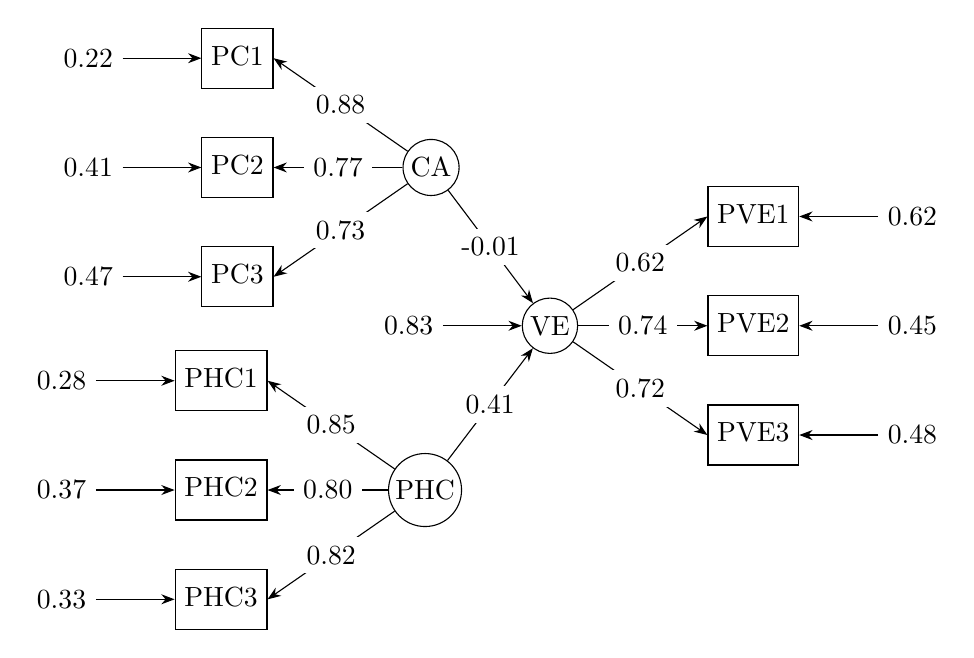
\begin{tikzpicture}
    [
    basic/.style={draw, text centered},
    circ/.style={basic, circle, minimum size=2em, inner sep=1.5pt},
    rect/.style={basic, text height=1em, text depth=.5em, minimum width=1.5em},
    >={Stealth[]}
    ]

    % Variables latentes
    \node [circ] (ve) {VE};
    \node [circ, above left=1.5cm and 1cm of ve] (ca) {CA};
    \node [circ, below left=1.5cm and 1cm of ve] (phc) {PHC};
    \draw [->] (ca) -- node[fill=white] {-0.01} (ve);
    \draw [->] (phc) -- node[fill=white] {0.41} (ve);
    % Variancia de VE
    \node [left=of ve] (delta) {0.83};
    \draw [->] (delta) -- (ve);
    % Variables indicadoras de VE
    \node [rect, above right=1cm and 2cm of ve.center] (pve1) {PVE1};
    \node [rect, right=2cm of ve.center] (pve2) {PVE2};
    \node [rect, below right=1cm and 2cm of ve.center] (pve3) {PVE3};
    \draw [->] (ve) -- node[fill=white] {0.62} (pve1.west);
    \draw [->] (ve) -- node[fill=white] {0.74} (pve2.west);
    \draw [->] (ve) -- node[fill=white] {0.72} (pve3.west);
    % Variancia de variables indicadoras de VE
    \node [right=of pve1] (epve1) {0.62};
    \node [right=of pve2] (epve2) {0.45};
    \node [right=of pve3] (epve3) {0.48};
    \draw [->] (epve1) -- (pve1);
    \draw [->] (epve2) -- (pve2);
    \draw [->] (epve3) -- (pve3);
    % Variables indicadoras de CA
    \node [rect, above left=1cm and 2cm of ca.center] (pc1) {PC1};
    \node [rect, left=2cm of ca.center] (pc2) {PC2};
    \node [rect, below left=1cm and 2cm of ca.center] (pc3) {PC3};
    \draw [->] (ca) -- node[fill=white] {0.88} (pc1.east);
    \draw [->] (ca) -- node[fill=white] {0.77} (pc2.east);
    \draw [->] (ca) -- node[fill=white] {0.73} (pc3.east);
    % Variancia de variables indicadoras de CA
    \node [left=of pc1] (epc1) {0.22};
    \node [left=of pc2] (epc2) {0.41};
    \node [left=of pc3] (epc3) {0.47};
    \draw [->] (epc1) -- (pc1);
    \draw [->] (epc2) -- (pc2);
    \draw [->] (epc3) -- (pc3);
    % Variables indicadoras de PHC
    \node [rect, above left=1cm and 2cm of phc.center] (phc1) {PHC1};
    \node [rect, left=2cm of phc.center] (phc2) {PHC2};
    \node [rect, below left=1cm and 2cm of phc.center] (phc3) {PHC3};
    \draw [->] (phc) -- node[fill=white] {0.85} (phc1.east);
    \draw [->] (phc) -- node[fill=white] {0.80} (phc2.east);
    \draw [->] (phc) -- node[fill=white] {0.82} (phc3.east);
    % Variancia de variables indicadoras de CA
    \node [left=of phc1] (ephc1) {0.28};
    \node [left=of phc2] (ephc2) {0.37};
    \node [left=of phc3] (ephc3) {0.33};
    \draw [->] (ephc1) -- (phc1);
    \draw [->] (ephc2) -- (phc2);
    \draw [->] (ephc3) -- (phc3);
  \end{tikzpicture}
  \caption{Modelo estimado sobre las habilidades cuantitativas}
  \label{fig:mod_teorico}
\end{figure}

\subsection{Simulación y estimación}

La simulación de los datos, junto con la estimación de los modelos, se realizó mediante el paquete \texttt{lavaan} \cite{lavaan} usando el software R \cite{R} mediante la interfaz gráfica de RStudio \cite{RStudio}. Para el manejo de bases de datos y demás visualizaciones fueron utilizados los paquetes \texttt{ggplot2} \cite{ggplot2}, \texttt{tidyr} \cite{tidyr}, \texttt{dplyr} \cite{dplyr}, \texttt{ggpubr} \cite{ggpubr}, \texttt{PerformanceAnalytics} \cite{PerformanceAnalytics} y \texttt{kableExtra} \cite{kableExtra}.

Para poder realizar la simulación deben seguirse varios pasos. Lo primero es definir el modelo teórico poblacional que van a seguir los datos simulados, como se describió en la sección anterior este modelo cuenta con dos variables exógenas y una endógena, cada una con tres variables indicadoras. Los datos se generan mediante la función \texttt{simulateData()} la cuál requiere especificar varios argumentos, uno de ellos es el modelo poblacional. Los otros dos argumentos a especificar son el tamaño de muestra deseado y el nivel de kurtosis de interés, la definición de estos escenarios se muestran en la Tabla \ref{tab:escenarios}:

\begin{table}[!h]
  \caption{\label{tab:unnamed-chunk-6}\label{tab:escenarios}Escenarios de simulación}
  \centering
  \resizebox{\linewidth}{!}{
    \fontsize{9}{11}\selectfont
    \begin{tabu} to \linewidth {>{\raggedleft}X>{\raggedleft}X>{\raggedleft}X>{\raggedleft}X>{\raggedleft}X>{\raggedleft}X>{\raggedleft}X>{\raggedleft}X>{\raggedleft}X>{\raggedleft}X}
      \toprule
      kurtosis                 & n  & kurtosis & n   & kurtosis & n   & kurtosis & n   & kurtosis & n                              \\
      \midrule
      \rowcolor{gray!6}  0.00  & 50 & 0.00     & 100 & 0.00     & 200 & 0.00     & 400 & 0.00     & 800                            \\
      0.62                     & 50 & 0.62     & 100 & 0.62     & 200 & 0.62     & 400 & 0.62     & 800                            \\
      \rowcolor{gray!6}  6.65  & 50 & 6.65     & 100 & 6.65     & 200 & 6.65     & 400 & 6.65     & 800                            \\
      21.41                    & 50 & 21.41    & 100 & 21.41    & 200 & 21.41    & 400 & 21.41    & 800                            \\
      \rowcolor{gray!6}  13.92 & 50 & 13.92    & 100 & 13.92    & 200 & 13.92    & 400 & 13.92    & 800                            \\
      \bottomrule
      \multicolumn{10}{l}{\textit{Fuente:} Elaboración propia a partir del estudio de la Universidad de California \cite{Gao2008}} \\
    \end{tabu}}
\end{table}

Con estos escenarios definidos, se generaron entonces, para cada combinación de tamaño de muestra y kurtosis un total de 2000 conjuntos de datos para cada uno. Una vez que se obtuvieron estos conjuntos de datos, el siguiente paso es realizar la estimación de los SEM con cada uno de ellos; para ello es necesario definir un modelo sin los valores de las cargas factoriales, pues se busca conocer las estimaciones a partir de los datos generados.

\subsection{Medidas de bondad de ajuste}

Las medidas de bondad de ajuste utilizadas para comparar el ajuste de los modelos, para cada uno de los escenarios de simulación son: el estadístico chi-cuadrado, el RMSEA, el SRMR y el CFI.

\subsubsection{Estadístico chi-cuadrado}

El estadístico de chi-cuadrado busca cuantificar la diferencia que se presenta entre la matriz de covariancias de una muestra con la matriz de covariancias estimadas mediante un cierto modelo. Según \citeasnoun{Hu1999}, su fórmula de cálculo viene dada por:
\[
  \chi^2 = (N-1) F_{min}
\]
donde \(N\) es el tamaño de la muestra y \(F_{min}\) es el mínimo obtenido mediante la función de ajuste, la cual, normalmente, se asume que es la distribución normal multivariada, utilizando el método de máxima verosimilitud. Este estadístico tiene una distribución chi-cuadrado con grados de libertad igual a la cantidad de piezas de información única en la matriz de covariancias menos la cantidad de parámetros a estimar del modelo, bajo el supuesto de normalidad y, si este supuesto no se cumple, la distribución asintótica sigue siendo una chi-cuadrado con esos mismos grados de libertad. El estadístico chi-cuadrado es muy utilizado en los modelos de ecuaciones estructurales y da origen a la gran mayoría de las demás medidas de ajuste utilizadas en dichos modelos, aunque puede presentar algunos problemas ya que depende del tamaño de la muestra, por lo que, con muestras grandes tiende a ser significativo, mientras que con muestras pequeños tiende a no ser significativo \cite{Kenny2015}.

\subsubsection{RMSEA}

El Error Cuadrático Medio de Aproximación (RMSEA por sus siglas en inglés) es una de las medidas de ajuste más conocidas y utilizadas en los modelos de ecuaciones estructurales. Su fórmula, según \citeasnoun{Hu1999}, viene dada por:
\[
  RMSEA = \sqrt{\max\left\{\frac{\chi^2 - gl}{gl (N-1)} , 0 \right\}}
\]
donde \(\chi^2\) es el valor de la chi-cuadrado, \(gl\) son los grados de libertad, y \(N\) es el tamaño de la muestra. Por lo general, se considera un valor del RMSEA menor a 0.05 como un indicador de un buen ajuste, mientras que un valor mayor a 0.1 representa un mal ajuste del modelo \cite{Kenny2015}.

\subsubsection{SRMR}

La Raíz Estandarizada del Error Cuadrático Medio (SRMR por sus siglas en inglés) es una medida de ajuste en la cual se comparan las diferencias entre las covariancias estimadas y las de la muestra. La fórmula de cálculo, con base en \citeasnoun{Hu1999} es:
\[
  SRMR = \sqrt{\left(2 \sum\limits_{i=1}^p \sum\limits_{j=1}^i \left((s_{ij} - \hat\sigma_{ij}) / (s_{ii} s_{jj}) \right)^2 \right)^2 / p(p+1)}
\]
donde \(p\) es el número de variables observadas, \(s_{ij}\) son las covariancias observadas y \(\hat\sigma_{ij}\) son las covariancias estimadas de las variables \(i\) y \(j\). Dado que se están comparando las covariancias observadas y las estimadas, un valor de 0 indica un ajuste perfecto del modelo, pero, por lo general, se considera un valor menor a 0.08 como un indicador de un buen ajuste \cite{Kenny2015}.

\subsubsection{CFI}

El Índice de Ajuste Comparativo (CFI por sus siglas en inglés) es una medida de ajuste que compara el valor de chi-cuadrado del modelo estimado con el valor de chi-cuadrado del modelo nulo, agregando una penalización por la cantidad de parámetros estimados. La fórmula de cálculo presentada por \citeasnoun{Hu1999} es la siguiente:
\[
  CFI = 1 - \left( \frac{\max \left\{(\chi^2_T - gl_T), 0  \right\}}{\max \left\{(\chi^2_T - gl_T), (\chi^2_N - gl_N), 0 \right\}} \right)
\]
donde \(\chi^2_T\) y \(\chi^2_N\) son los valores del estadístico chi-cuadrado para el modelo estimado y el nulo, respectivamente, y \(gl_T\) y \(gl_N\) son los grados de libertad de los modelos estimado y nulo, respectivamente. Esta medida de ajuste puede tomar un valor entre 0 y 1 y se considera que el modelo tiene un buen ajuste cuando es mayor a 0.95, un buen ajuste cuando el valor está entre 0.9 y 0.95 y un mal ajuste cuando es menor que 0.9 \cite{Kenny2015}.

\section{Results}

\subsection{Introducción}

\section{Conclusions}

\subsection{Introducción}

\subsection{Conclusiones}

\subsection{Recomendaciones}

\section{Appendices}

\bibliography{mybibfile}

\appendix

\end{document}